\documentclass{astroedu-lab}

\begin{document}

\pagestyle{plain}

\begin{problem}{\huge Радиотехническая работа 24\\\\Безынерционные линейные цепи\\\\Выполнил Жданов Елисей Б01-205}

\section{Оборудование:}

Макетная плата

Набор резисторов различных номиналов

Электронный осциллограф на печатной плате

Электронный генератор сигналов на печатной плате

\section{Задание}

\subsection{Делитель напряжения}

\begin{figure}[!h]
	\centering
	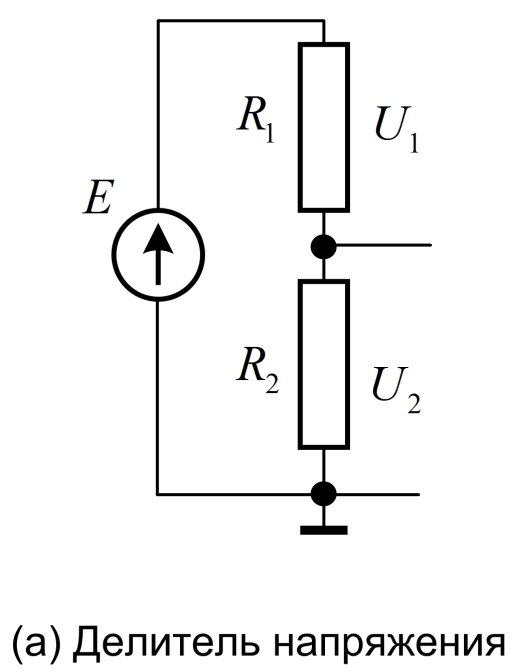
\includegraphics[width=0.25\textwidth]{16a.png}
	\label{fig:boiler}
\end{figure}

\subsubsection{Теория}

В схеме делителя напряжения на рис. 16 напряжение $E$ идеального источника делится на части $U_1, U_2\left(U_1+U_2=E\right)$, падающие на резисторах $R_1, R_2$.

Делитель - это распространенное схемное решение для преобразования источника питания $E$ в источник опорного напряжения с требуемым эквивалентным напряжением $E^*=E \frac{R_2}{R_1+R_2}$ и внутренним сопротивлением $R^*=\frac{R_1 R_2}{R_1+R_2}=R_1 \| R_2$, равным параллельному соединению сопротивлений $R_1, R_2$.

Делитель естественным образом возникает, когда источник во внутренним сопротивлением $R_1$ подключается к нагрузке $R_2$, рис. 16 . Это сопровождается потерей уровня сигнала источника, выражаемой коэффициентом передачи $K=\frac{u}{e}=\frac{R_2}{R_1+R_2}$.

\subsubsection{Выполнение}

1. Соберем заданную схему на макетной плате. Подключим центральный узел схемы к измерительной ноге платы - генератора.

Для схемы были выбраны резисторы $R_1$ = 3 кОм, а $R_2$ = 12 кОм(из пропорции $\frac{E-E^*}{R_1}=\frac{E^*}{R_2}$).

Теоретически выбранное значение напряжения $E^*=2 \mathrm{~B}$, практически же  $E^*=2.056 \mathrm{~B}$. Различие действительно мало с учетом погрешности сопротивлений подобранных резисторов. Подаваемое значение напряжения питания $E=10 \mathrm{~B}$.

\begin{figure}[!h]
	\centering
	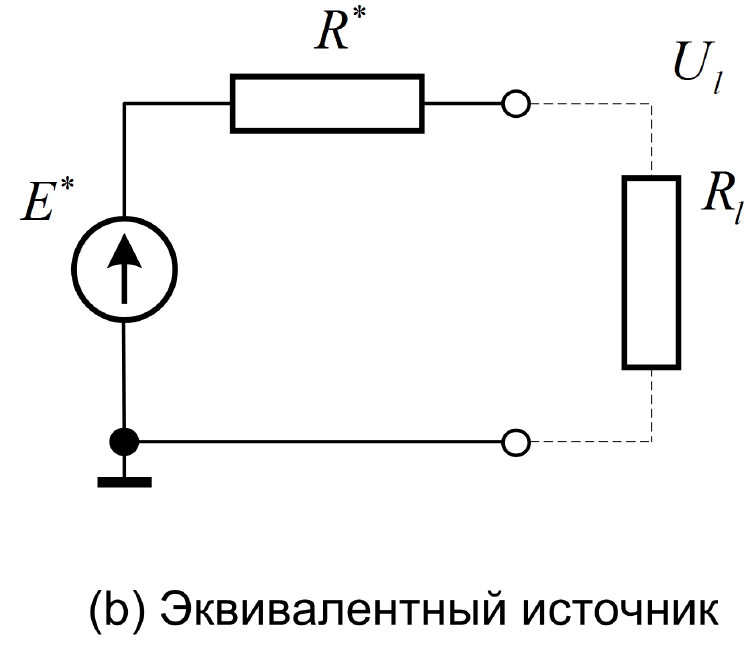
\includegraphics[width=0.32\textwidth]{16b.png}
	\label{fig:boiler}
\end{figure}

Внутреннее сопротивление определим по методу двух нагрузок: измерим напряжение холостого хода на выходе делителя $U_{o c}=E^*=2.056 \mathrm{~B}$ и напряжение $U_l=0.9473 \mathrm{~B}$ на дополнительно подключенном резисторе нагрузки $R_l*=2$ кОм, см рисунок $16 \mathrm{b}$. Внутреннее сопротивление $R^*$ оценим из пропориции
$$
\frac{E^*-U_l}{R^*}=\frac{U_l}{R_l}
$$

Итого $R^*$ = 2.34 кОм. Теоретическое значение же равно $R^*$ = 2.4 кОм, что тоже довольно близко.

\begin{figure}[!h]
	\centering
	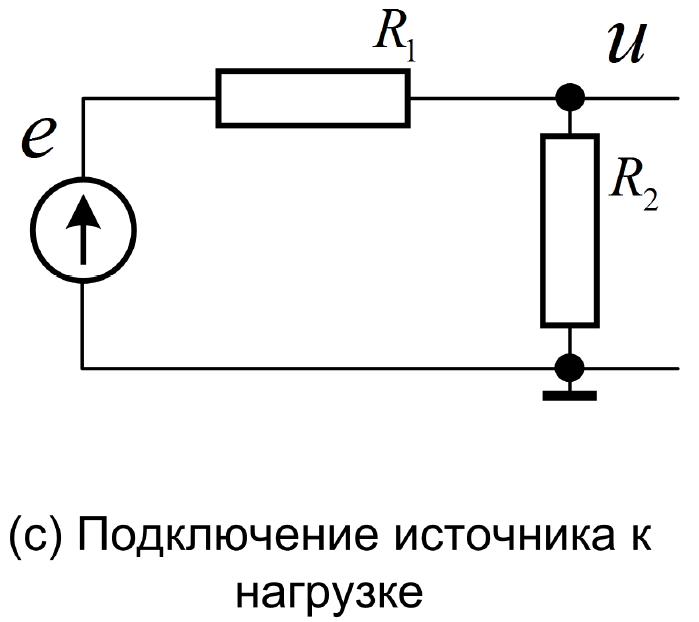
\includegraphics[width=0.3\textwidth]{16c.png}
	\label{fig:boiler}
\end{figure}

2. Подадим а вход делителя синусоидальное напряжение $е = 1.02 \mathrm{~B}$ от лабораторного источника. На основании эффективного значения напряжения $u = 200.5 \text{ мВ}$, рассчитаю коэффициент передачи $K=\frac{u}{e} = 0.1966$, что почти равно теоретическому значению $K=\frac{u}{e} = 0.2$.

\subsubsection{Вывод}

Проведенные эксперименты подтверждают полученные теоретические выкладки. Разница между получаемыми теоретическими и практическими величинами почти постоянна и составляет около 2-3$\%$, что позволяет определить её как точность маркировки номиналов резисторов.

\subsection{Параллельный сумматор}

\subsubsection{Теория}

\begin{figure}[!h]
	\centering
	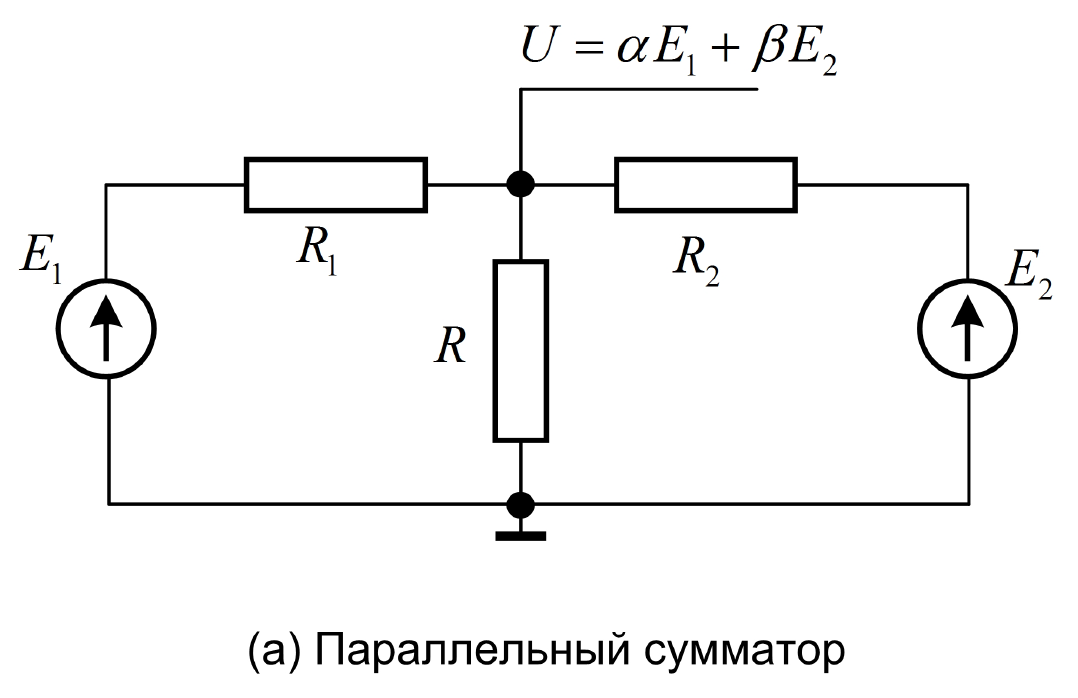
\includegraphics[width=0.45\textwidth]{17a.png}
	\label{fig:boiler}
\end{figure}

Схема на рисунке реализует параллельный сумматор, выход U которого является взвешенной суммой входных напряжений $E_1$ и $E_2$ с коэффициентами $\alpha$ и $\beta$

\begin{equation}
	U = \alpha E_1 + \beta E_2
\end{equation}

Приравняв к нулю напряжение $E_2$ (короткое замыкание на выходе) легко увидеть что $\alpha$ - это коэффициент передачи делителя напряжения на резисторах $R_1$ и $\left(R \| R_2\right)$ : $\alpha=\frac{R \| R_2}{R_1+R \| R_2}$. Аналогично, $\beta=\frac{R \| R_1}{R_2+R \| R_1}$.
15
Замена левого и правого источников напряжения эквивалентными источниками тока приводит к эквивалентной схеме на рис. $17 \mathrm{~b}$

\begin{figure}[!h]
	\centering
	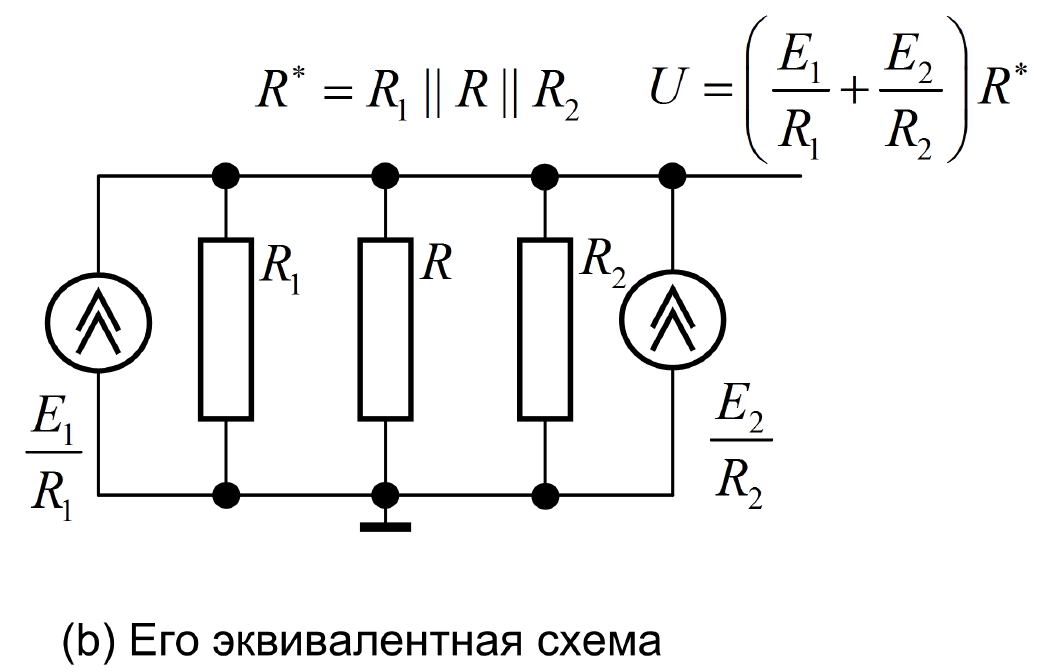
\includegraphics[width=0.47\textwidth]{17b.png}
	\label{fig:boiler}
\end{figure}

Из схемы становится ясно, что
$$
\frac{\alpha}{\beta}=\frac{R_2}{R_1} ; \quad \alpha+\beta=\frac{1}{1+\frac{R_1 \| R_2}{R}},
$$
а сопротивление эквивалентного источника составляет $R^*=R_1\|R\| R_2$.

\subsubsection{Выполнение}

1. Выберем компоненты сумматора по заданным весовым коэффициентам $\alpha=0.4$, $\beta=0.2$. Резистор $R_1$ возьмем номиналом 1.8 кОм. Резистор $R_2$ определить из соотношения $\frac{R_2}{R_1}=\frac{\alpha}{\beta}=2$, то бишь 3.6 кОм. Наконец, номинал резистора $R$ из соотношения

$$
\alpha+\beta=0.6=\frac{1}{1+\frac{R_1 \| R_2}{R}}
$$

составит 1.8 кОм.

2. Соберем схему сумматора на макетной плате. Подадим синусоидальное напряжение с заданной амплитудой $2 \mathrm{~B}$ на вход $E_1$ и постоянное напряжение $+5 \mathrm{~B}$ на вход $E_2$. На осциллографе уровень постоянной и амплитуду переменной составляющих в суммарном сигнале составит $U_{\verb!_!} = 1.12$ В и $U_{\verb!~!} = 0.765$ В соответственно. Тогда коэффициенты $\alpha = 0.3825$ и $\beta = 0.224$.

Для реализации метода двух нагрузок подключу схему к постоянному току, и присоединю к узлам схемы резистор номиналом 2 кОм. Значение $U_l = 3.7$ В при напряжении $E_2 = 5$ В, а значит $R^* = 700$ Ом, что довольно близко к теоретическому значению $R^* = 720$ Ом.

\subsubsection{Вывод}

Больше всего от теоретического значения отличается значение $\alpha$ (порядка $10\%$), что объяснимо неточностью номинала резистора и прочими неучтенными факторами. Зато остальные значение отличаются от теоретических меньше чем на $5\%$, что является хорошим совпадением.

\subsection{H-параметры}

\subsubsection{Теория}

\begin{figure}[!h]
	\centering
	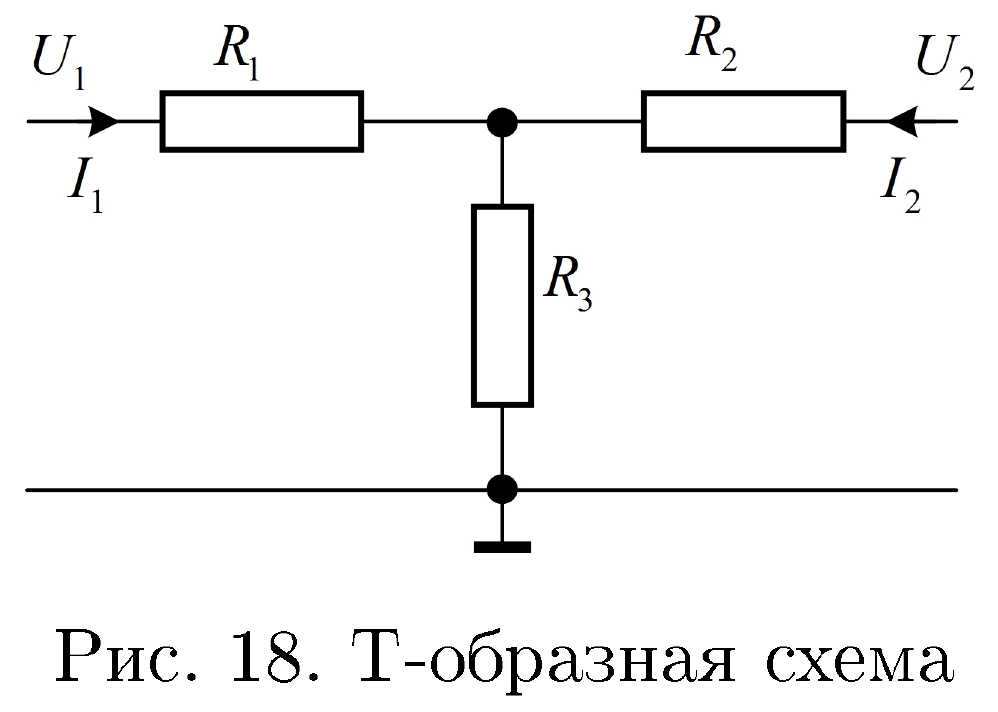
\includegraphics[width=0.35\textwidth]{18.png}
	\label{fig:boiler}
\end{figure}

1. Для схемы на рисунке приведены формулы для $H$-параметров.
$$
\left(\begin{array}{c}
U_1 \\
I_2
\end{array}\right)=\left(\begin{array}{ll}
h_{11} & h_{12} \\
h_{21} & h_{22}
\end{array}\right)\left(\begin{array}{c}
I_1 \\
U_2
\end{array}\right)=\left(\begin{array}{cc}
R_1+R_3 \| R_2 & \frac{R_3}{R_3+R_2} \\
\frac{R_3}{R_3+R_2} & \frac{1}{R_3+R_2}
\end{array}\right)\left(\begin{array}{c}
I_1 \\
U_2
\end{array}\right) .
$$

Для выбранных значений номиналов резисторов, напряжений и токов значения параметров

$$
\left(\begin{array}{ll}
h_{11} = 2200 \text{ Ом} & h_{12} = 0.6 \\
h_{21} = 0.6 & h_{22} = 0.2 \cdot 10^{-3} \text{ См}
\end{array}\right)
$$

\subsubsection{Выполнение}

\begin{figure}[!h]
	\centering
	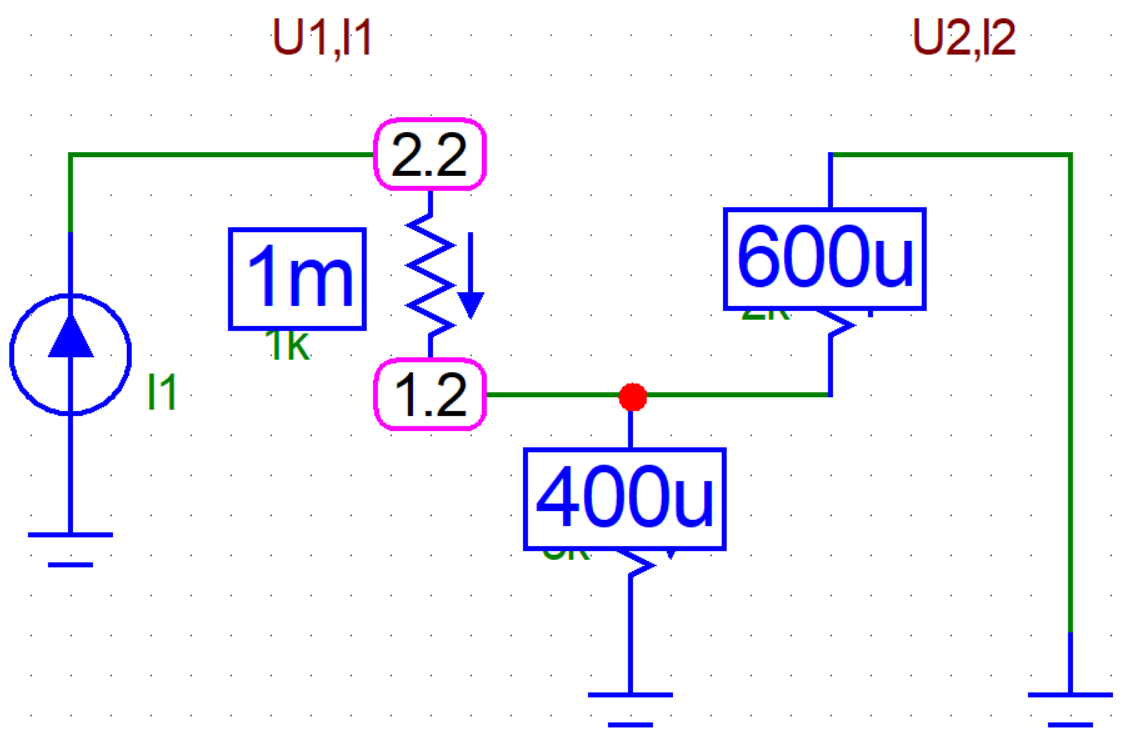
\includegraphics[width=0.4\textwidth]{18a.png}
	\label{fig:boiler}
\end{figure}

2. В программе Мicro-Сар по схеме выше с коротким замыканием на выходе $\left(U_2=0\right)$ и источником тока $I_1$ на входе измерим $U_1 = 2.2$ В$, I_2 = 600$ мкА и вычислим $h_{11}=\frac{U_1}{I_1} = 2200 $ Ом, $h_{21}=\frac{I_2}{I_1} = 0.6$.

\begin{figure}[!h]
	\centering
	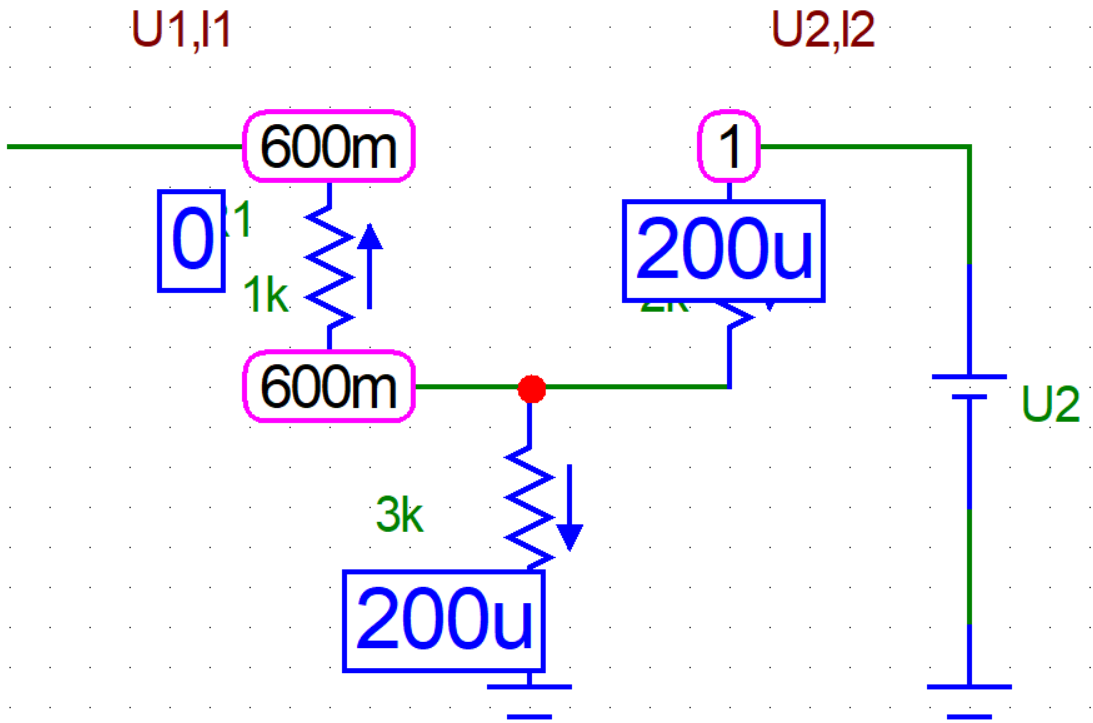
\includegraphics[width=0.4\textwidth]{18b.png}
	\label{fig:boiler}
\end{figure}

По второй схеме с холостым входом на входе и источником напряжения $U_2$ на выходе измерим $U_1, I_2$ и вычислим $h_{12}=\frac{U_1}{U_2} = 0.6, h_{22}=\frac{I_2}{U_2} = 0.2 \cdot 10^{-3}$ См. Показатели тождественны теории.

\subsubsection{Вывод}

Теоретическая модель верна

\subsection{Звезда и треугольник}

\subsubsection{Теория}

\begin{figure}[!h]
	\centering
	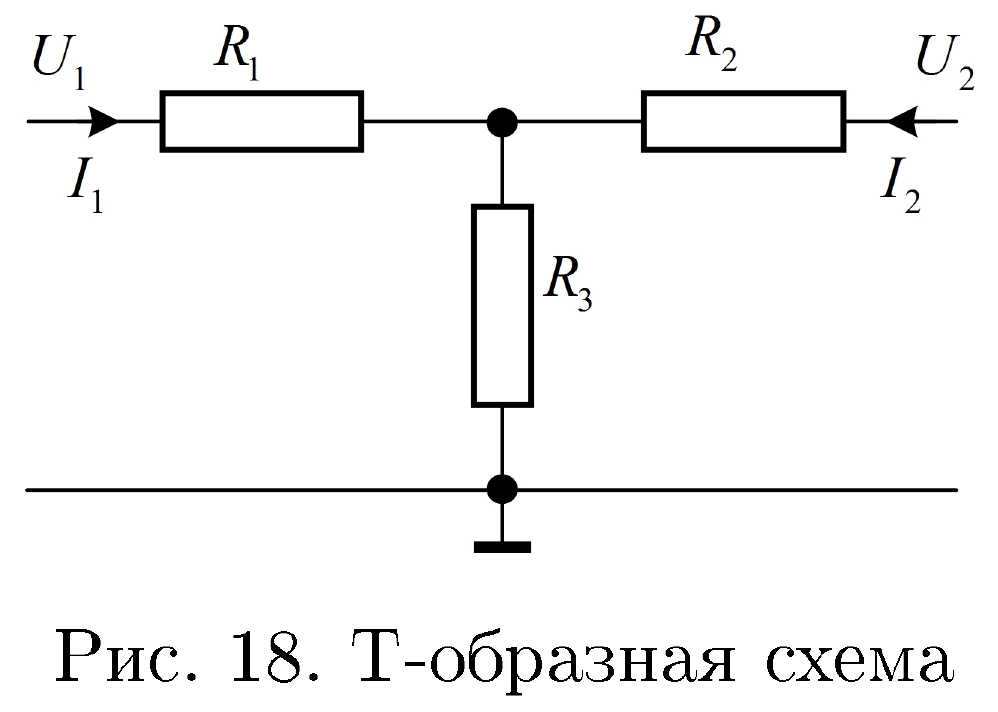
\includegraphics[width=0.35\textwidth]{18.png}
	\label{fig:boiler}
\end{figure}

1. Для схемы на рисунке приведены формулы для $X$-параметров.
$$
\left(\begin{array}{l}
U_1 \\
U_2
\end{array}\right)=\left(\begin{array}{ll}
X_{11} & X_{12} \\
X_{21} & X_{22}
\end{array}\right)\left(\begin{array}{l}
I_1 \\
I_2
\end{array}\right)=\left(\begin{array}{cc}
R_1+R_3 & R_3 \\
R_3 & R_2+R_3
\end{array}\right)\left(\begin{array}{l}
I_1 \\
I_2
\end{array}\right) .
$$

Для выбранных значений резисторов, напряжений и токов значения параметров

$$
\left(\begin{array}{ll}
X_{11} = 4 \text{ кОм} & X_{12} = 3 \text{ кОм} \\
X_{21} = 3 \text{ кОм} & X_{22} = 5 \text{ кОм}
\end{array}\right)
$$

\subsubsection{Выполнение}

\begin{figure}[!h]
	\centering
	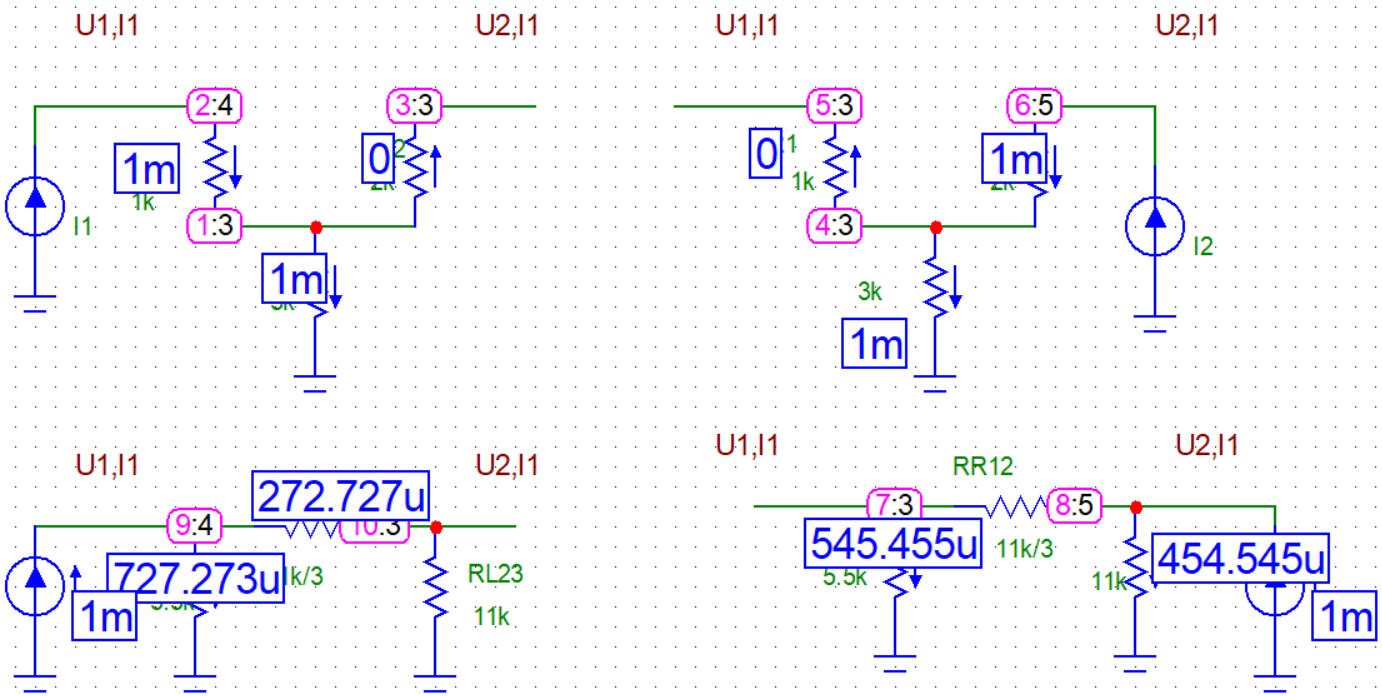
\includegraphics[width=0.9\textwidth]{18c.png}
	\label{fig:boiler}
\end{figure}

2.

Открыть файл храг.cir. Пересчитать параметры представленной там звезды в параметры треугольника:
$$
R_{13}=R_1+R_3+\frac{R_1 R_3}{R_2} = 5.5 \text{ кОм}, \quad R_{12}=R_1+R_2+\frac{R_1 R_2}{R_3} = \frac{11}{3} \text{ кОм}, \quad R_{23}=R_2+R_3+\frac{R_2 R_3}{R_1} = 11 \text{ кОм} .
$$

В программе Мicro-Сар установим вычисленные значения резисторов в схемы с треугольниками.

По левой схеме $I_2=0$ измерим напряжения $U_1 = 4 \text{ В}, U_2 = 3 \text{ В}$ и вычислим $X_{11}=\frac{U_1}{I_1} = 4 \text{ кОм}, X_{21}=\frac{U_2}{I_1} = 3 \text{ кОм}$. По правой с $I_1=0$ измерим $U_1 = 3 \text{ В}, U_2 = 5 \text{ В}$ и вычислим $X_{12}=\frac{U_1}{I_2} = 3 \text{ кОм}$, $X_{22}=\frac{U_2}{I_2} = 5 \text{ кОм}$.

\subsubsection{Вывод}

Теоретические значения совпали с моделированием, значит, теория верна.

\subsection{Лестничные структуры}

\subsubsection{Теория}

\begin{figure}[!h]
	\centering
	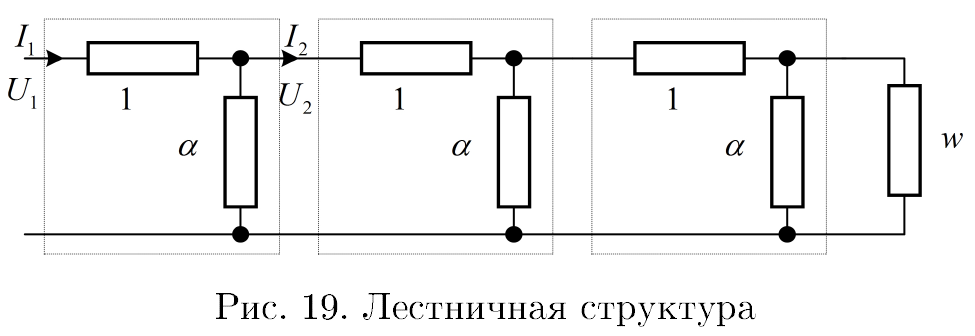
\includegraphics[width=0.6\textwidth]{19.png}
	\label{fig:boiler}
\end{figure}

Передаточная матрица блока лестничной структуры с резисторами $R_1=1$ и $R_2=\alpha$ легко вычисляется
$$
\left(\begin{array}{c}
U_2 \\
I_2
\end{array}\right)=\left(\begin{array}{ll}
A_{11} & A_{12} \\
A_{21} & A_{22}
\end{array}\right)\left(\begin{array}{c}
U_1 \\
I_1
\end{array}\right)=\left(\begin{array}{cc}
1 & -1 \\
-\frac{1}{\alpha} & \frac{1+\alpha}{\alpha}
\end{array}\right)\left(\begin{array}{c}
U_1 \\
I_1
\end{array}\right) .
$$
Подстановка значений $A$-параметров в
$$
A_{11}+\frac{A_{12}}{w}=A_{21} w+A_{22}=\gamma
$$
дает уравнение $w^2-w-\alpha=0$ для характеристического сопротивления и значение $\gamma=\frac{w-1}{w}$ для коэффициента передачи напряжения/тока при характеристической нагрузке. Положительное значение характеристического сопротивления составляет
$$
w=\frac{1+\sqrt{1+4 \alpha}}{2} .
$$
Имеется ряд значений $\alpha$, при которых характеристическое сопротивление вычисляется без радикала
$$
\left(\alpha=2, w=2, \gamma=\frac{1}{2}\right), \quad\left(\alpha=6, w=3, \gamma=\frac{2}{3}\right), \quad\left(\alpha=12, w=4, \gamma=\frac{3}{4}\right) .
$$

\newpage

\subsubsection{Выполнение}

1. Рассмотрим в Micro-cap четырехзвенную лестничную схему с $\alpha=2, \gamma=\frac{1}{2}$, нагруженную на характеристическое сопротивление $w=2$ кОм. На схеме приведены результаты моделировани напряжений и токов.

\begin{figure}[!h]
	\centering
	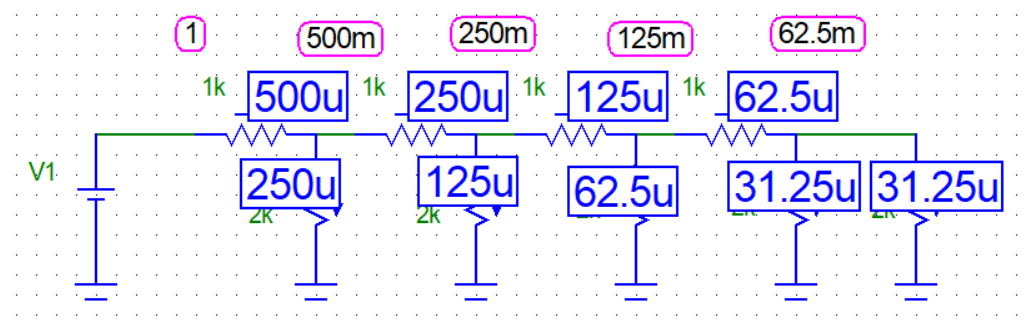
\includegraphics[width=0.7\textwidth]{19a.png}
	\label{fig:boiler}
\end{figure}

Согласно матрице, $\frac{U_1}{U_2} = 2 = \frac{I_1}{I_2}$, что видно на моделировании. В дальнейшем, все результаты также будут сходиться с теоретическим расчетом, который, из очевидности, будет опушен.

2. Повторим это исследование при $\alpha=6, \gamma=\frac{2}{3}$, установив на схеме номиналы четырех вертикальных резисторов $R_{2 j}=6$ кОм и нагрузки $w=3$ кОм.

\begin{figure}[!h]
	\centering
	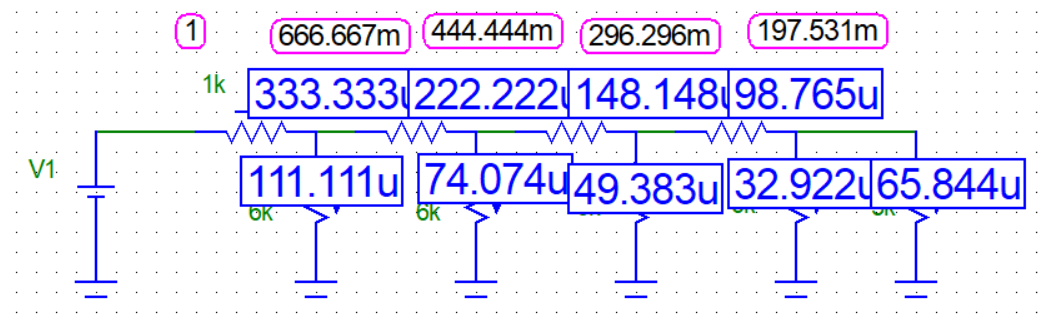
\includegraphics[width=0.7\textwidth]{19b.png}
	\label{fig:boiler}
\end{figure}

3. Проделаем это для $\alpha=12, \gamma=\frac{3}{4}\left(R_{2 j}=12\right.$ кОм, $w=4$ кОм $)$ и для $\alpha=1, \gamma=\frac{\sqrt{5}-1}{\sqrt{5}-1}=0.38$ $\left(R_{2 j}=1, w=\frac{1+\sqrt{5}}{2}=1.618\right.$ кOм $)$.

\begin{figure}[!h]
	\centering
	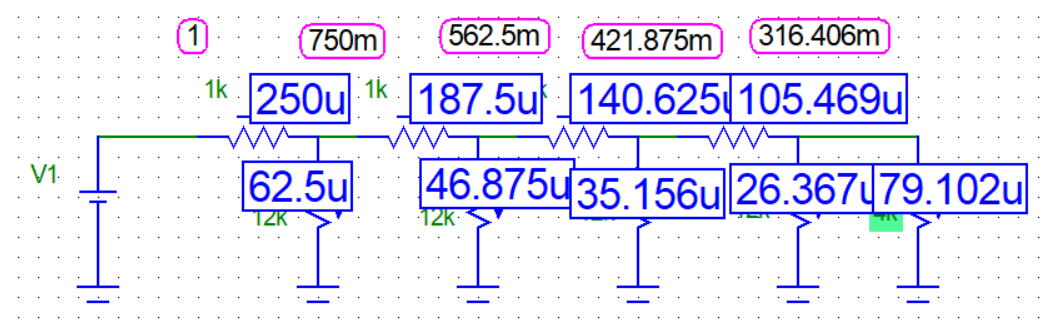
\includegraphics[width=0.7\textwidth]{19c.png}
	\label{fig:boiler}
\end{figure}

\begin{figure}[!h]
	\centering
	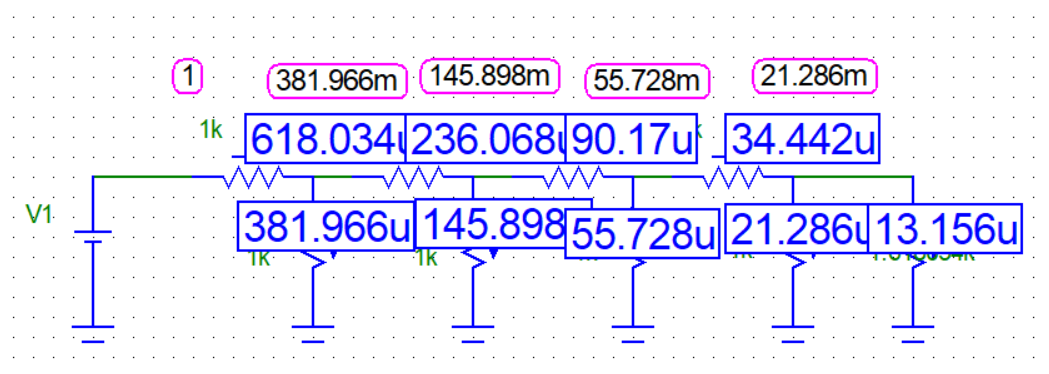
\includegraphics[width=0.7\textwidth]{19d.png}
	\label{fig:boiler}
\end{figure}

4. Из предыдущих схем следует вполне обоснованная реализация делителя напряжения, который в зависимости от подаваемого на ножки вертикальных резисторов напряжения U, будет выдавать на ноге входа напряжение V, причем оно будет логично зависеть от суперпозиции токов, протекающих через резисторы. 

Рассмотрим схему 4-разрядного цифро-аналогового преобразователя (ЦАП), который преобразует двоичный позиционный код $\left(X_3, X_2, X_1, X_0\right)$ в пропорциональное напряжение
$$
\text { OUT }=X_3 2^3+X_2 2^2+X_1 2^1+X_0 .
$$
Снимем зависимость напряжения $O U T$ от двоичного кода $\left(X_3, X_2, X_1, X_0\right)$, изменяя его в диапазоне от $(0,0,0,0)=0$ до $(1,1,1,1)=15$.

Очевидно, что напряжение на выходе будет равно десятичной записи двоичного кода на ключах, т.е. прямая пропорциональность y=x.

Теоретические выкладки полностью подтвердились на моделировании.

Примеры преобразования приведены ниже

\begin{figure}[!h]
	\centering
	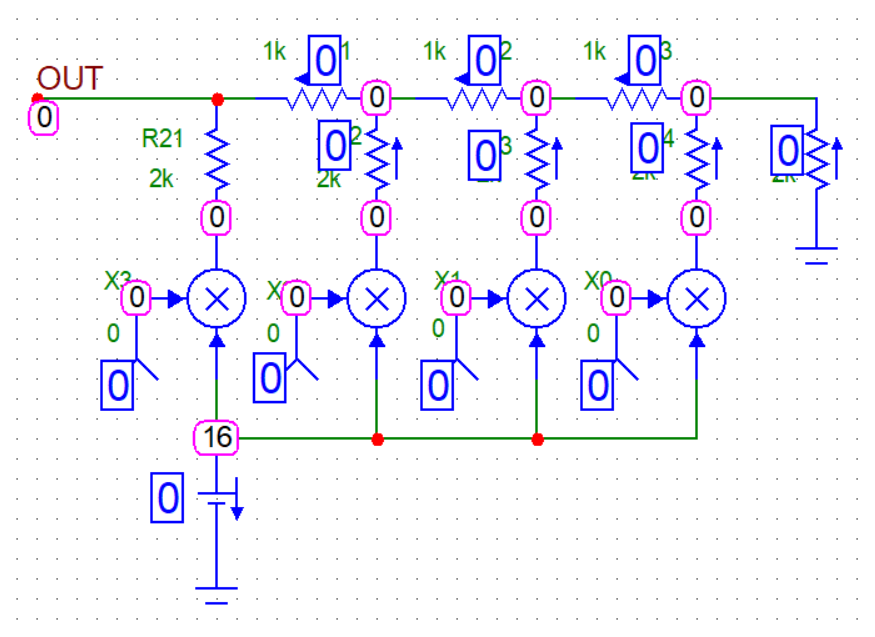
\includegraphics[width=0.7\textwidth]{19e.png}
	\label{fig:boiler}
\end{figure}

\begin{figure}[!h]
	\centering
	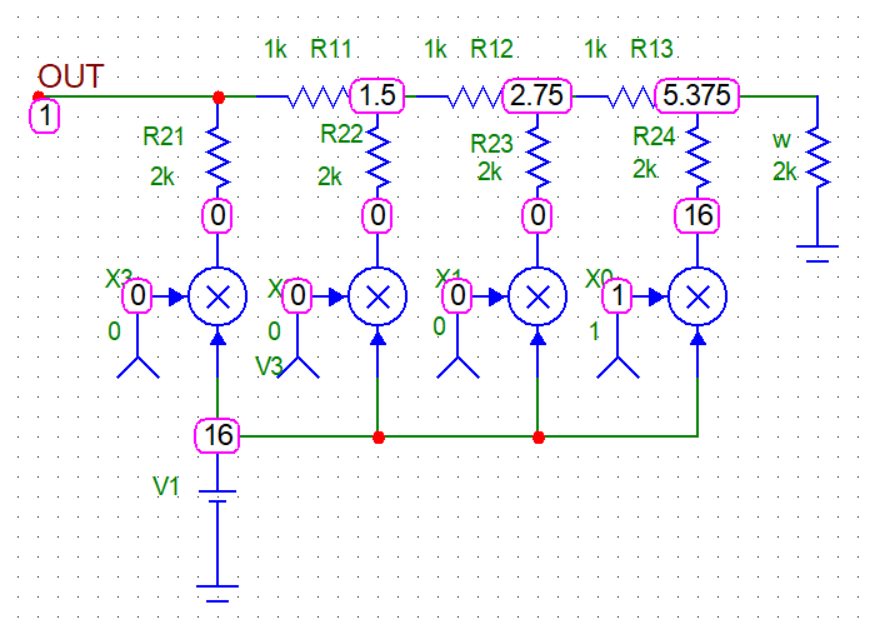
\includegraphics[width=0.7\textwidth]{19g.png}
	\label{fig:boiler}
\end{figure}

\begin{figure}[!h]
	\centering
	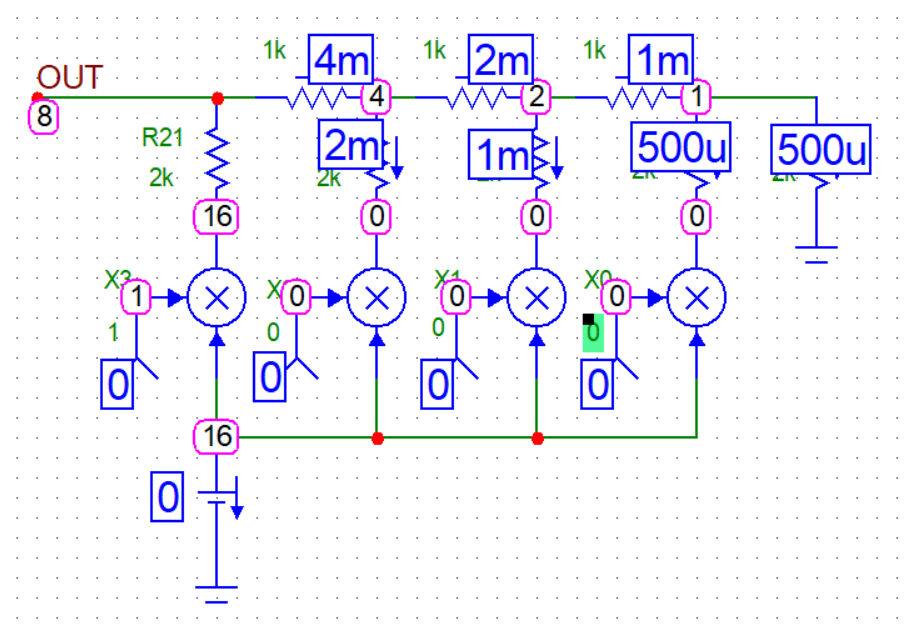
\includegraphics[width=0.7\textwidth]{19h.png}
	\label{fig:boiler}
\end{figure}

\newpage

\section{Вывод}

Результаты моделирования, как и ожидается, тождественны теории, в то время как замеры на макетной плате незначительно от нее отличаются. Все это позволяет сказать, что использованные методы расчета и анализа безинерционных линейных цепей дают хорошие результаты в области применимости.


\end{problem}
\end{document}